\section{Ejercicio 3}

\subsection{Descripci\'on del problema} \label{ej_3:descripcion}

El problema se trata de un juego que forma parte de un reality show. Este juego tiene un campo de juego cuadrado dividido en celdas, de tamano n x n. Cada una de estas celdas posee un resorte con el que se puede saltar hacia otras celdas. Estos resortes var\'ian en sus potencias, siendo la potencia la cantidad de celdas que pueden propulsar al jugador. Es posible apuntar los resortes hacia adelante, atr\'as, izquierda y derecha. Adicionalmente cada jugador posee unidades extra de potencia, que le permiten potenciar sus saltos.  \'Estan son limitadas, y el jugador las podr\'a usar a elecci\'on en los saltos que le parezcan convenientes.

\vspace{2mm}

Un ejemplo de salto ser\'ia la siguiente situaci\'on: vemos que la celda tiene una potencia de 1, por lo que el jugador podr\'ia saltar una celda izquierda, hacia adelante o hacia la derecha. Y en caso de que quisiera usar una potencia, podr\'ia saltar does celdas hacia adelante, pero su reserva de potencias se reducir\'ia en uno.
 \vspace{2mm}

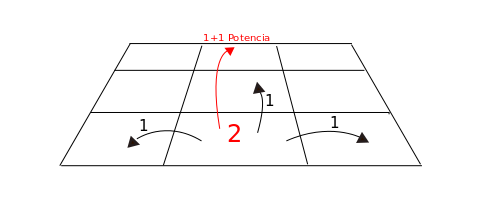
\includegraphics[scale=0.8]{images/saltos}

El objetivo del juego es llegar de una celda origen a otra destino, realizando la menor cantidad de saltos posibles. Por esto, se pide el diseno e implementaci\'on de un algoritmo que calcule y de como resultado uno de los caminos que lleguen de origen a destino cuya cantidad de saltos sea m\'inima.
\vspace{2mm}


El algoritmo tiene que tener una complejidad de $O(n^3*k)$, con $n$ la cantidad de filas y columnas del campo de juego y $k$ la cantidad de potencias otorgadas al inicio del juego al jugador.
\vspace{2mm}
\subsection{Ideas para la resoluci\'on} \label{ej_3:idea}

Decidimos encarar la resolucio\'on como un problema de grafos. El campo de juego es representado como un grafo con un nodo por cada celda, y las aristas son orientadas, de peso constante y representan todos los posibles saltos entre celda y celda. 

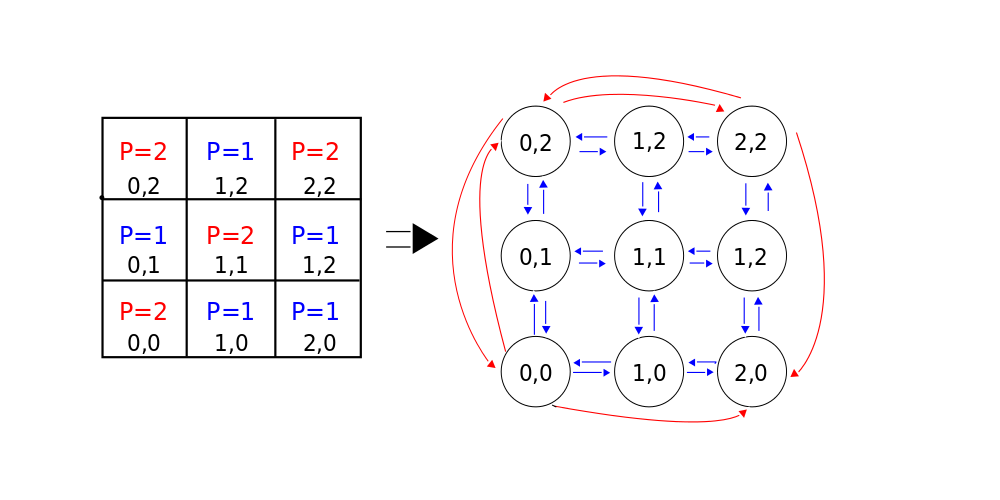
\includegraphics[scale=0.5]{images/grafo1}

\vspace{2mm}


Por cada uno de los valores $0..k$ de potencia tenemos un campo de juego de los anteriormente mencionados. Los vamos a llamar $"niveles"$, y van a ser subgrafos interconectados para formar un grafo general que va a resolver el problema. Entre estos niveles va a haber aristas conectando los nodos de mayor nivel con los de menor nivel, representando el hecho de $"gastar"$ potencias, es decir, si en un turno estoy en el nivel $k$ y utilizo dos potencias, en el siguiente turno voy a estar posicionado en un nodo del nivel $k-2$.

\vspace{2mm}

De esta forma, estar en el nodo $(i,j)$ del nivel $k$ representa estar posicionado en la celda de juego $(i,j)$ y disponer de $k$ potencias para utilizar .Podemos $"saltar \: entre \: celdas"$, movi\'endonos de un nodo a otro usando las aristas este nivel. En caso de querer usar las potencias, debemos movernos por aristas que conectan los nodos de nivel $k$ con los niveles inferiores. Por ejemplo, si estamos en el nodo $(i,j,k)$, de potencia 2, y queremos saltar 3 nodos hacia la derecha, debemos tomar la arista orientada que nos lleva al nodo $(i+3,j,k-1)$ (en caso de disponer de una potencia). De esto deducimos que las aristas entre niveles s\'olo salen de nodos de nivel superior hacia nodos de nivel inferior. Formalicemos esto:

\vspace{2mm}

Para cada nivel, sea:

\begin{align*}
G_L = (V_L, E_L) /\: V_ = {V_{1_{L}},..., V_{n_{L}}} =  \{ casillas \: 1..n  \:con \: L \: potencias \: disponibles \}
\end{align*}
\vspace{2mm}
Por lo tanto, el grafo $G$ es:

\begin{align*}
G = (W, A) /\: W \: =  \:\cup_{i=1}^{k} V_i(G_i) \: \land \: A \: = \: (\cup_{L=1}^{k} E_L(G_L)) \cup T
\end{align*}

\vspace{2mm}

Donde $T$ son las aristas entre niveles, descriptas a continuaci\'on:

\vspace{2mm}

Se tienen aristas dirigidas en cada nivel tal que si $v, u \in V_t$, $(u,v) \in E_t$ sii $v$ es alcanzable desde $u$ sin usar potencias.
Dados niveles $G_m,\, G_j\, /\, m\,< \,j$ y dos v\'ertices $v \in V_m(G_m) \: \land \: w \in V_j(G_J)$ existe una arista dirigida $"entre"$ niveles, que pertenezca a $T$, sii $w$ es alcanzable desde $v$ usando estrictamente $(j-m)$ unidades de potencia, es decir, que la distancia en casillas (verticales u horizontales) de $v$ a $w$ es igual a $(j-m) + pot(v)$.

\vspace{2mm}

En el siguiente diagrama mostramos las aristas entre niveles que deber\'ian tomarse en caso de usar una potencia en las celdas $(0,2)$ y $(2,0)$

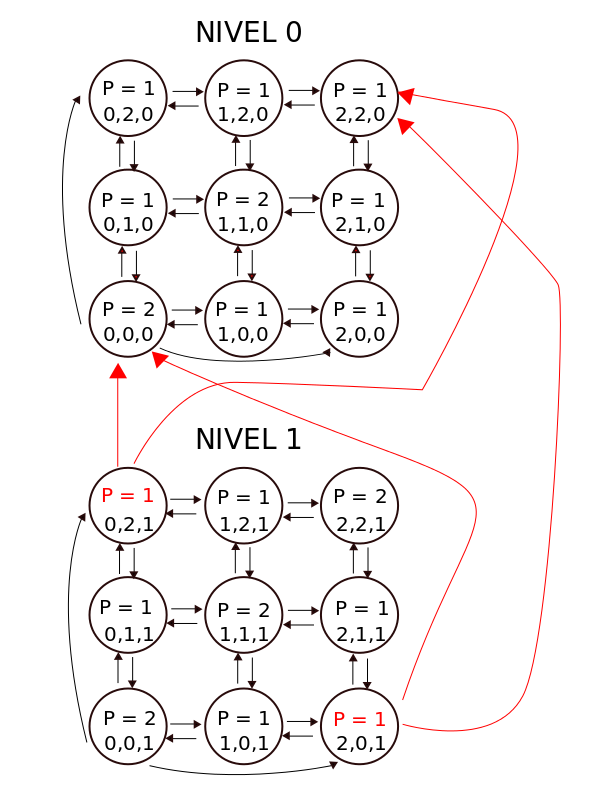
\includegraphics[scale=0.5]{images/dospisos}

\vspace{2mm}

Notemos que al avanzar hacia niveles m\'as bajos no se puede ir hacia arriba (lo cual tiene sentido pues el nivel actual indica la cantidad de potencias disponibles para usar, y este valor nunca puede aumentar)

\vspace{2mm}

Definimos $n_0$ como el nodo origen $/ n_0 \in V_k$ (primer nivel, m\'as alto), dado por las coordenadas cartesianas de la celda de comienzo de la entrada. Si la celda destino en el juego es $(i,j)$ definimos el conjunto de nodos destino como los nodos $(i,j,k)$, con $k$ entre 0 y la cantidad de potencias m\'axima, de forma que al llegar al nodo destino $(i,j,l)$, l es la cantidad de potencias sin usar.

\vspace{2mm}

Las aristas son de peso constante en su totalidad (en particular, 1). Adem\'as, en cada arista se guarda un valor indicando la cantidad de niveles atravesadas en este paso, lo cual es equivalente a la cantidad de potencias utilizadas en el salto. No confundir este valor con el costo o peso de la arista.
\vspace{2mm}
(Dibujo zarpado)
\vspace{2mm}

De esta forma, encontrar el camino que realize la menor cantidad de saltos se reduce a buscar el camino m\'as corto en el grafo de $n_0$ a alg\'un nodo destino, guardando en cada caso el valor de cada arista (potencia usada) y la posici\'on $(i,j)$ del nodo sin importar el nivel actual. Un recorrido de anchura BFS del grafo nos brinda el camino m\'as corto, comenzando la b\'usqueda desde $n_0$.

\subsection{Estructuras de datos}

A cada una de las celdas, las representamos con la clase $nodo$, que posee tres atributos: $x$, $y$ y $level$, (el numero de fila y columna de la celda que representa este nodo, y el nivel en el que se encuentra el nodo).

\vspace{2mm}

Representamos el grafo en memoria con una modificaci\'on del m\'etodo de listas de adyacencia. La estructura es un diccionario (java $HashMap$)

\subsubsection{Algoritmo} \label{ej_3:algoritmo}


\subsection{Cota de complejidad} \label{ej_3:cota}

\subsection{Casos de prueba y resultado del programa} \label{ej_3:casos}

\subsection{Mediciones de performance} \label{ej_3:performance}

\subsection{Concluciones} \label{ej_3:concluciones}

